\section{評価実験}
\subsection{実験設定}
提案手法の有効性を確認するために，以下 2 つのデータ
セットで評価実験を行った．
\begin{enumerate}[1.]
  \item シミュレーションデータセット (CARLA\cite{13})
  \item 公開データ (KITTI-360 データセット\cite{14})
\end{enumerate}

どちらのデータセットにおいても，PMOD-NetDと，以下3つの手法と比較する．
\begin{enumerate}[1.]
  \item PMOD-Net\cite{3}
  \item NDDepth\cite{1}
  \item MIMDepth\cite{2}
\end{enumerate}

NDDepthとMIMDepthはKITTIデータセットで高い精度を
出しており，事前学習済みのモデルも公開されているため，
比較手法として用いることにした．学習済みのモデルが公
開されているため，KITTI-360データセットではスケール調
整不要で距離精度の比較が可能である．CARLAで使用する場
合は式(\ref{metric_Id})のようにスケール調整した結果で比較する．ここ
では2.0[m]の位置にカメラを設置した．
\subsection{使用データセット}
シミュレーションデータセットは，自動運転研究用シミュレ
ータである CARLA\cite{13}を用いて作成した．CARLAには特徴の異
なる7種類のマップがあり，マップごとにランダムに配置され
た人や車を含むデータセットを作成した．学習データには各マ
ップから600枚ずつ，合計4200枚を使用し，テストには各マッ
プから学習に使用していない1840 枚ずつ，合計12880 枚を用
いた．\reffig{ex_CARLA}に学習および評価に使用した画像例を示す．三次
元地図の投影にはシミュレータが出力するカメラ位置を用いた．
公開データセットとしてKITTI-360\cite{14}を使用した．ドイツ
郊外を撮影した大規模な車載センサデータセットであり，9つ
のシーケンスを提供している．本実験ではデータ数が少ないシ
ーケンス03を除いた8シーケンスの三次元地図と左カメラ画
像を使用した．学習データには各シーケンスから500枚ずつ，
合計4000枚を使用し，テストには学習に使用していないデー
タをすべて用いた．テスト時にはKITTI-360が提供している自
己位置誤差を含んだ慣性航法システムのデータを使用し，実際
の位置誤差を想定した実験を行った．

\subsection{評価指標}
評価は画像中の動的障害物に対して行う．本実験では人と車
を動的障害物とした．距離推定の評価指標には，距離誤差平均
を示すMAEを用いる．MAEは式(\ref{MAE})で計算する．$n$は評価対象の
領域を示す画素数であり,$i$は画素位置である．$D_P$は各手法が推
定した距離画像，$D_{GT}$は正解の距離画像である．ともにカメラか
ら各物体までの距離を示す．また方向性のあ
る誤差を評価するため，式(\ref{MAE})において絶対値内の値が正の場合と負の場合だけを評価した
値をそれぞれ ME+，ME-として分けて評価する．
\begin{equation}
  \label{MAE}
  MAE= \frac{1}{n}{}\sum_{i=1}^{n}|D_P(i)-D_{GT}(i)|
\end{equation}
\begin{figure}[t]
  \centering
  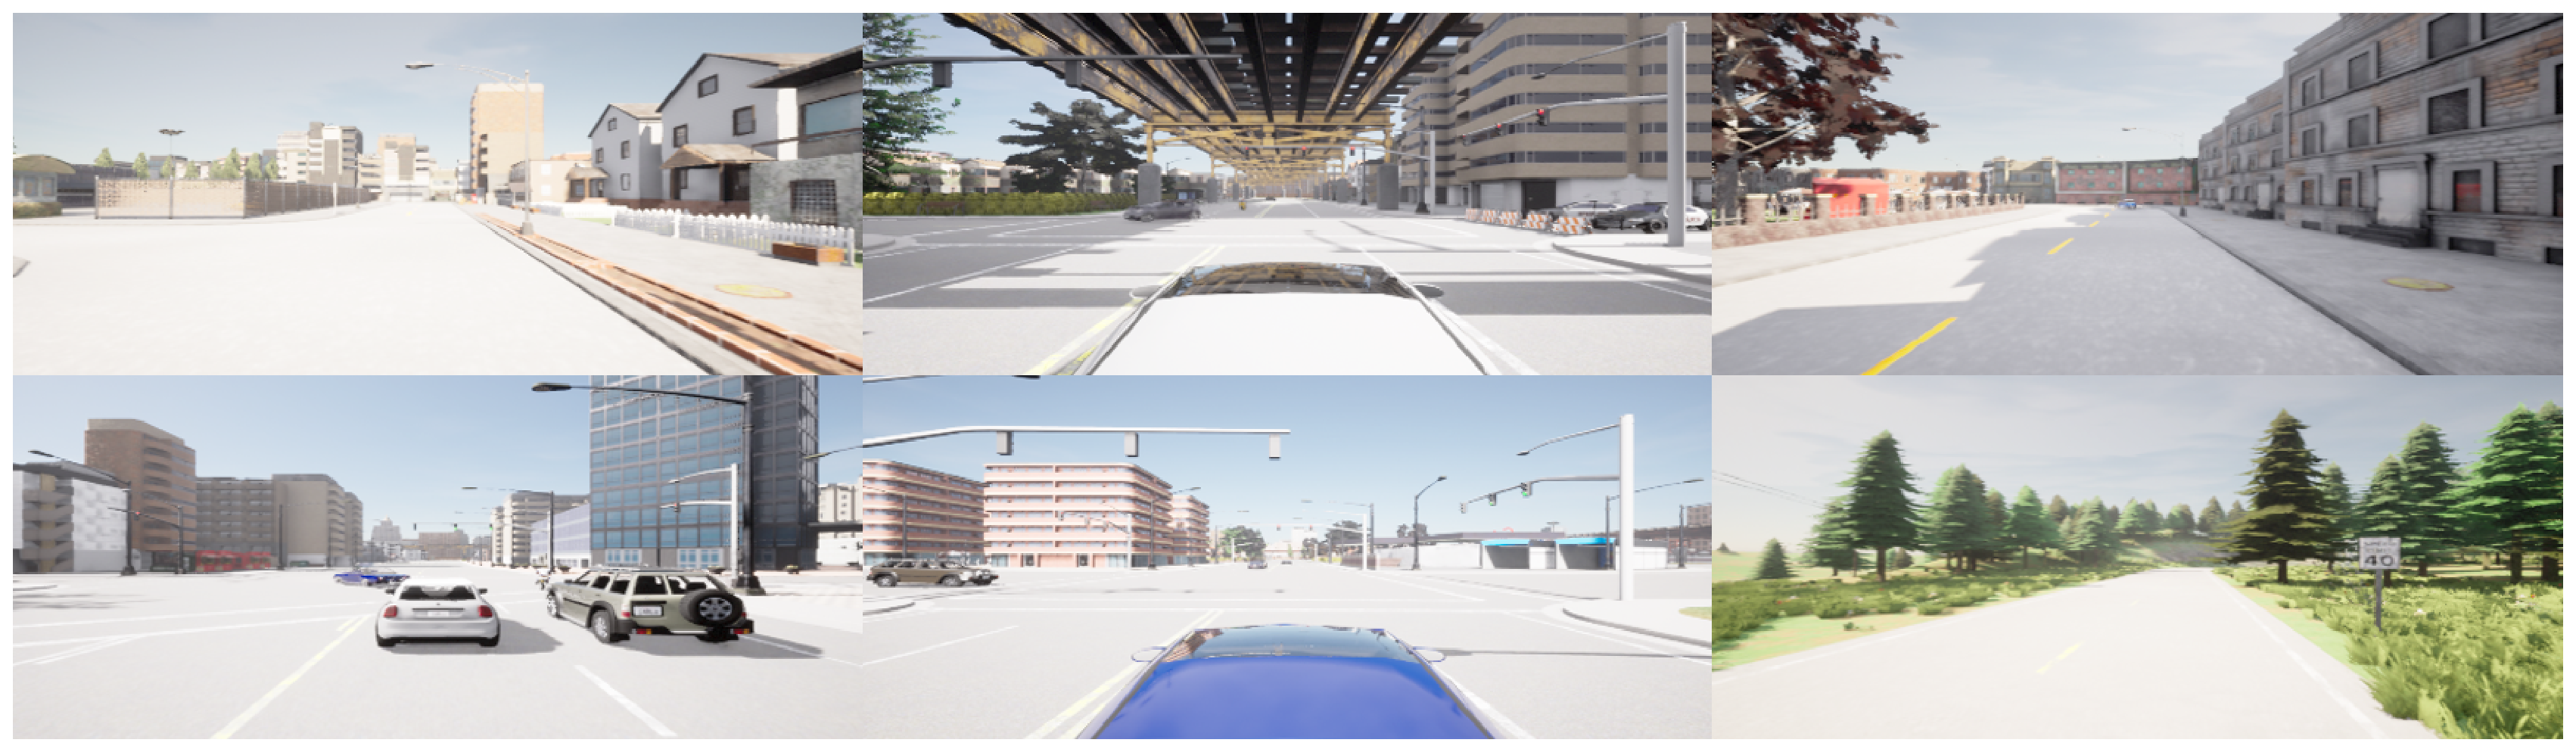
\includegraphics[width=0.9\linewidth]{img/evaluation/CARLA_ex.eps}
  \caption{Examples in CARLA}
  \label{ex_CARLA} 
\end{figure}
\begin{table}[t]
  \centering
  \caption{MAE [m] in CARLA}
  \label{result_MAE_CARLA}
  \begin{tabular}{c|cccc}
      \toprule
      Method                                       & Vehicle            & Person                   \\ \midrule
      PMOD-Net\cite{3}                             & 1.19          & 3.01                 \\ \midrule
      NDDepth\cite{1}                                   & 4.08          & 3.57                 \\ \midrule
      MIMDepth\cite{2}                                    & 3.63          & 3.13                 \\ \midrule
      PMOD-NetD (NDDepth\cite{1})                                  & 1.12          & 2.52                 \\ \midrule
      PMOD-NetD (MIMDepth\cite{2})                                   & $\bm{1.09}$          & $\bm{2.39}$                 \\ \bottomrule
      \end{tabular}
\end{table}
\begin{table}[t]
  \centering
  \caption{MAE [m] in KITTI-360}
  \label{result_MAE_KITTI-360}
  \begin{tabular}{c|cccc}
      \toprule
      Method                                       & Vehicle            & Person         \\ \midrule
      PMOD-Net\cite{3}                                      & 2.27         & 4.10        \\ \midrule
      NDDepth\cite{1}                                            & 4.00         & 4.91        \\ \midrule
      MIMDepth\cite{2}                                             & 4.00         & 4.98        \\ \midrule
      PMOD-NetD (NDDepth\cite{1})                                           & 1.99         & 3.29        \\ \midrule
      PMOD-NetD (MIMDepth\cite{2})                                            & $\bm{1.97}$         & $\bm{3.25}$        \\ \bottomrule
      \end{tabular}
\end{table}
\begin{table}[t]
  \centering
  \caption{{ME [m] in CARLA}}
  \label{result_ME_CARLA}
  \begin{tabular}{c|cc|cc}
      \toprule
      \multirow{2}{*}{Method}  & \multicolumn{2}{c}{Vehicle} & \multicolumn{2}{c}{Person} \\ \cmidrule{2-5} 
                                             & ME+            & ME-          & ME+           & ME-         \\ \midrule
      PMOD-Net\cite{3}                             & 0.571          & -0.423         & 2.52         & -1.76        \\ \midrule
      NDDepth\cite{1}                                   & 2.88          & -2.79         & 2.30          & -5.51        \\ \midrule
      MIMDepth\cite{2}                                    & 2.68          & -1.96         & 1.99          & -5.16        \\ \midrule
      PMOD-NetD                                  & \multirow{2}{*}{0.544}          & \multirow{2}{*}{-0.450}         & \multirow{2}{*}{2.05}          & \multirow{2}{*}{-1.26}        \\ 
      (NDDepth\cite{1})                        &                                  &                                  &                                  &                                 \\ \midrule
      PMOD-NetD                                   & \multirow{2}{*}{$\bm{0.479}$}          & \multirow{2}{*}{$\bm{-0.382}$}         & \multirow{2}{*}{$\bm{1.95}$}          & \multirow{2}{*}{$\bm{-1.23}$}        \\
      (MIMDepth\cite{2})&                                  &                                  &                                  &                                 \\ \bottomrule
    \end{tabular}
\end{table}
\begin{table}[t]
  \centering
  \caption{ME [m] in KITTI-360}
  \label{result_ME_KITTI-360}
  \begin{tabular}{c|cc|cc}
    \toprule
    \multirow{2}{*}{Method}  & \multicolumn{2}{c}{Vehicle} & \multicolumn{2}{c}{Person} \\ \cmidrule{2-5} 
                                           & ME+            & ME-          & ME+           & ME-         \\ \midrule
    PMOD-Net\cite{3}                             & 0.637         & -0.857         & 2.05         & -1.34        \\ \midrule
    NDDepth\cite{1}                                   & 1.40         & -1.27         & 2.02         & -2.76        \\ \midrule
    MIMDepth\cite{2}                                    & 1.43         & -1.26         & 2.09         & -2.78        \\ \midrule
    PMOD-NetD                                  & \multirow{2}{*}{$\bm{0.397}$}          & \multirow{2}{*}{-0.766}         & \multirow{2}{*}{1.02}          & \multirow{2}{*}{-1.38}        \\ 
    (NDDepth\cite{1})                        &                                  &                                  &                                  &                                 \\ \midrule
    PMOD-NetD                                   & \multirow{2}{*}{0.414}          & \multirow{2}{*}{$\bm{-0.751}$}         & \multirow{2}{*}{$\bm{0.942}$}          & \multirow{2}{*}{$\bm{-1.29}$}        \\
    (MIMDepth\cite{2})&                                  &                                  &                                  &                                 \\ \bottomrule
  \end{tabular}
\end{table}
% \begin{table}[t]
%   \centering
%   \caption{ME [m]}
%   \label{result_ME}
%   \begin{tabular}{cc|cc|cc}
%       \toprule
%       \multirow{2}{*}{Method} & \multirow{2}{*}{Class} & \multicolumn{2}{c}{CARLA} & \multicolumn{2}{c}{KITTI-360} \\ \cmidrule{3-6} 
%                          &                    & ME+            & ME-          & ME+           & ME-         \\ \midrule
%       \multirow{2}{*}{PMOD-Net\cite{3}}                  & Vehicle           & 0.571          & -0.423         & 0.637         & -0.857        \\
%                         & Person                  & 2.52          & -1.76         & 2.05         & -1.34        \\ \midrule
%       \multirow{2}{*}{NDDepth\cite{1}}                 & Vehicle                  & 2.88          & -2.79         & 1.40         & -1.27        \\
%                         & Person                  & 2.30          & -5.51         & 2.02         & -2.76        \\ \midrule
%       \multirow{2}{*}{MIMDepth\cite{2}}                  & Vehicle                  & 2.68          & -1.96         & 1.43         & -1.26        \\
%                         & Person                 & 1.99          & -5.16         & 2.09         & -2.78        \\ \midrule
%       \multirow{2}{*}{D}                 & Vehicle                 & 0.544          & -0.450         & $\bm{0.397}$         & -0.766        \\
%                         & Person                 & 2.05          & -1.26         & 1.02         & -1.38        \\ \midrule
%       \multirow{2}{*}{E}                  & Vehicle                 & $\bm{0.479}$          & $\bm{-0.382}$         & 0.414         & $\bm{-0.751}$        \\
%                         & Person                 & $\bm{1.95}$          & $\bm{-1.23}$         & $\bm{0.942}$         & $\bm{-1.29}$        \\ \bottomrule
%       \end{tabular}
% \end{table}
\subsection{実験結果と考察}
各データセットにおける結果を\reftable{result_MAE_CARLA}，\reftable{result_MAE_KITTI-360}，\reftable{result_ME_CARLA}，\reftable{result_ME_KITTI-360}に示す．\reffig{result_CARLA}，\reffig{result_KITTI-360}は，
Segmentation結果と推定距離画像から作成した点群の鳥瞰図である．
\begin{figure}[t]
  \centering
  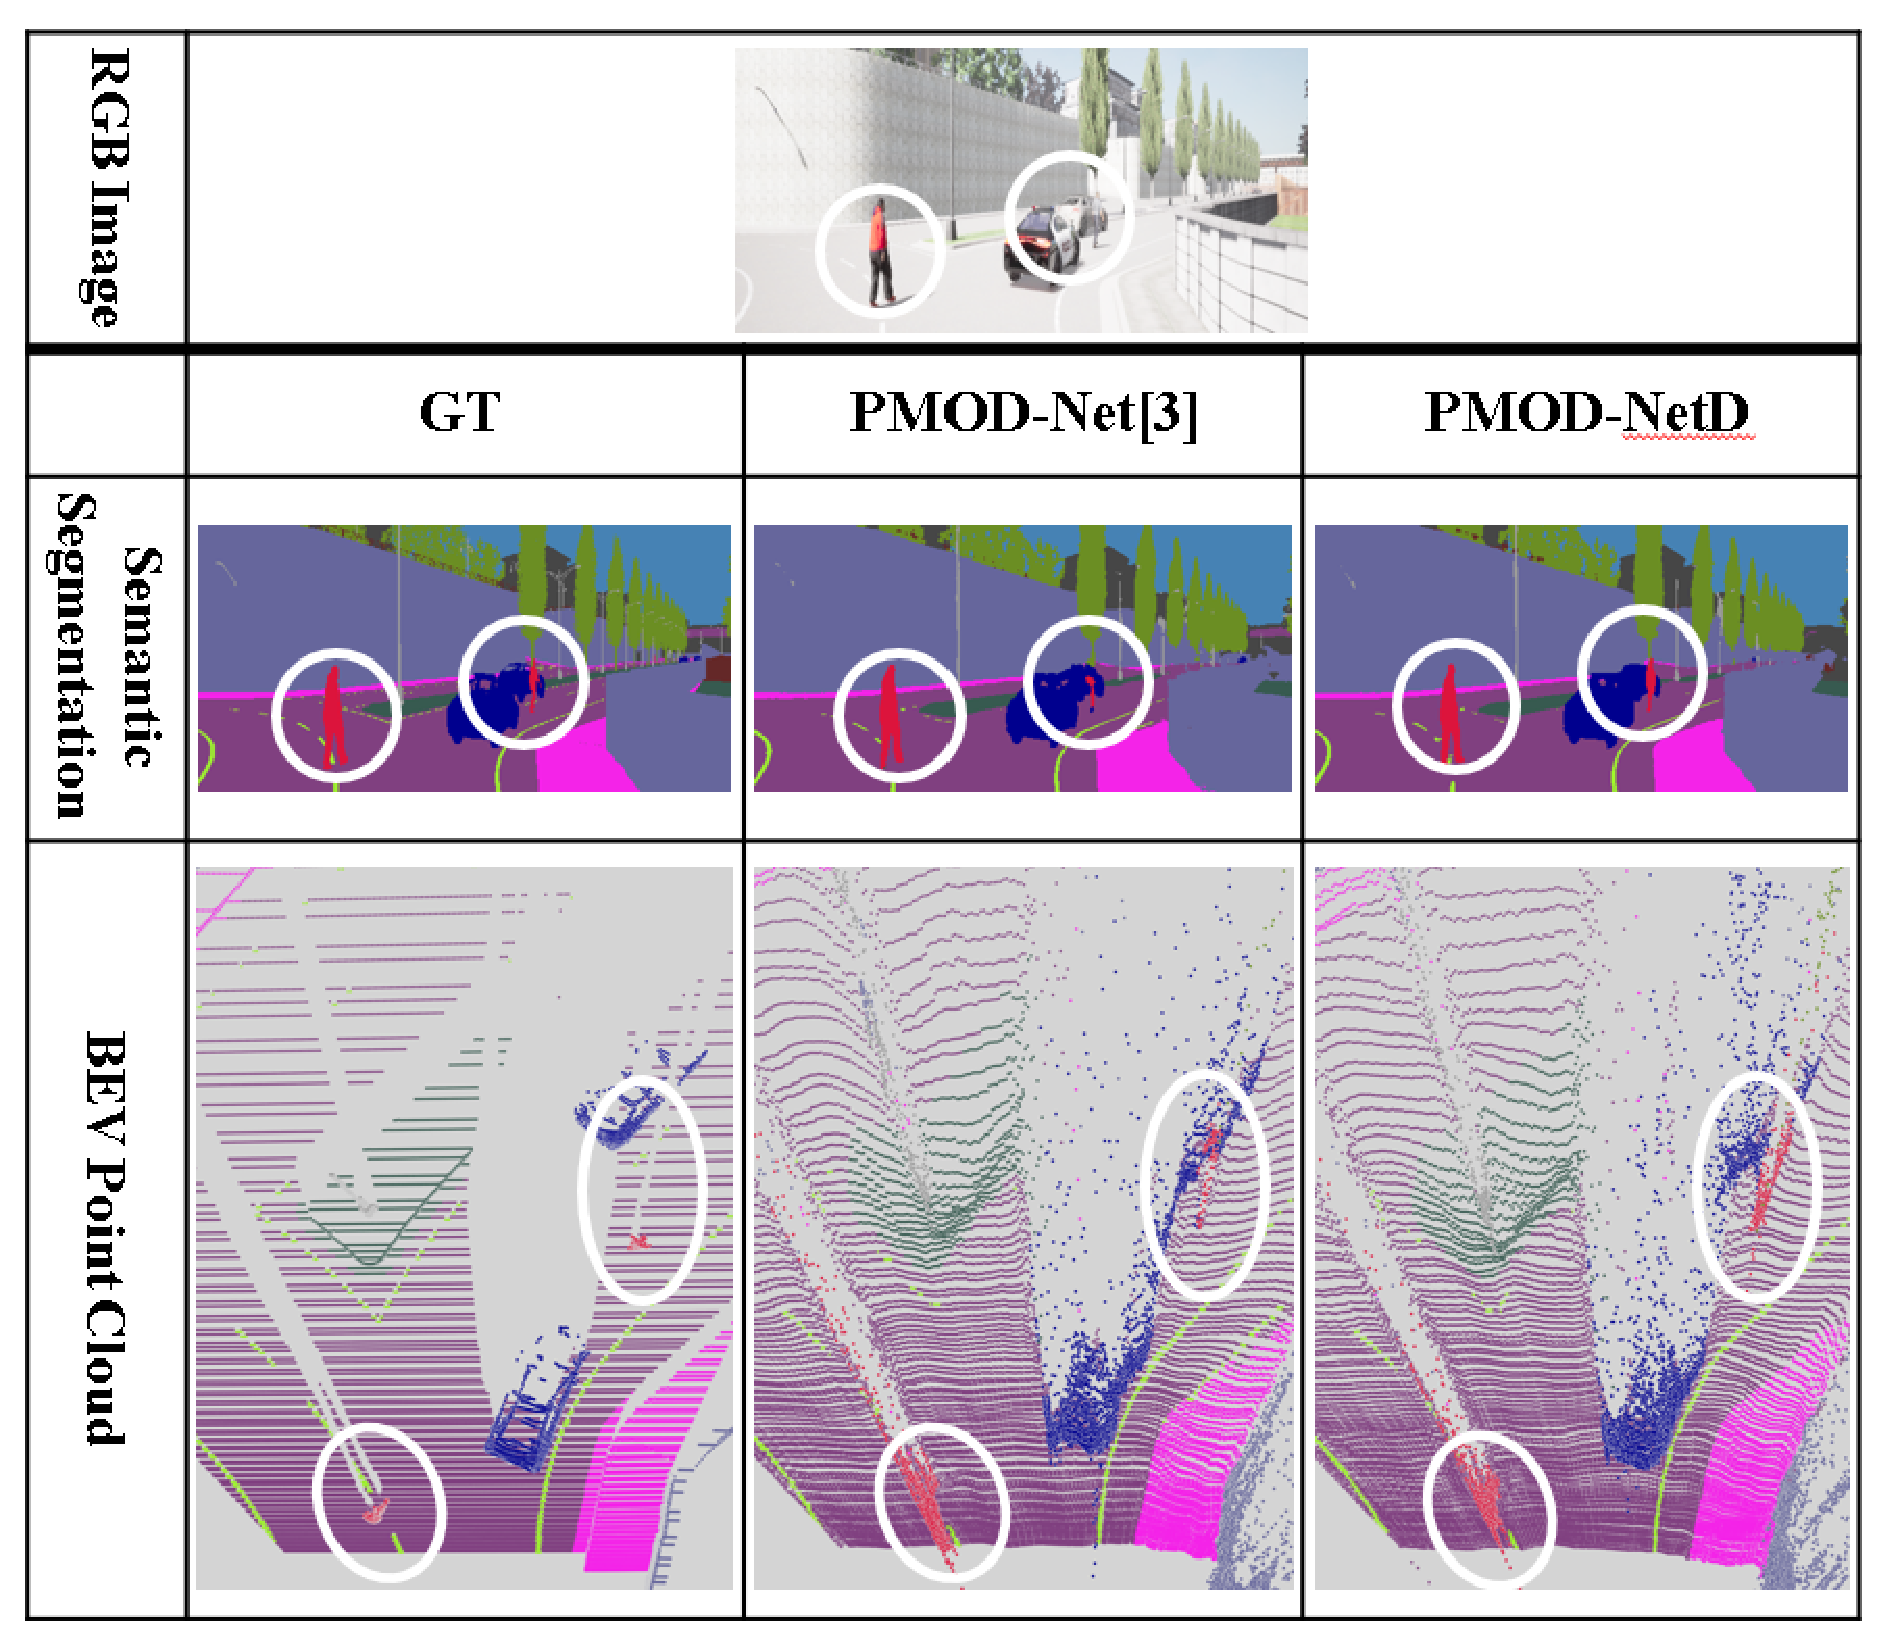
\includegraphics[width=0.935\linewidth]{img/evaluation/result_CARLA.eps}
  \caption{Experimental results in CARLA}
  \label{result_CARLA} 
\end{figure}
\begin{figure}[t]
  \centering
  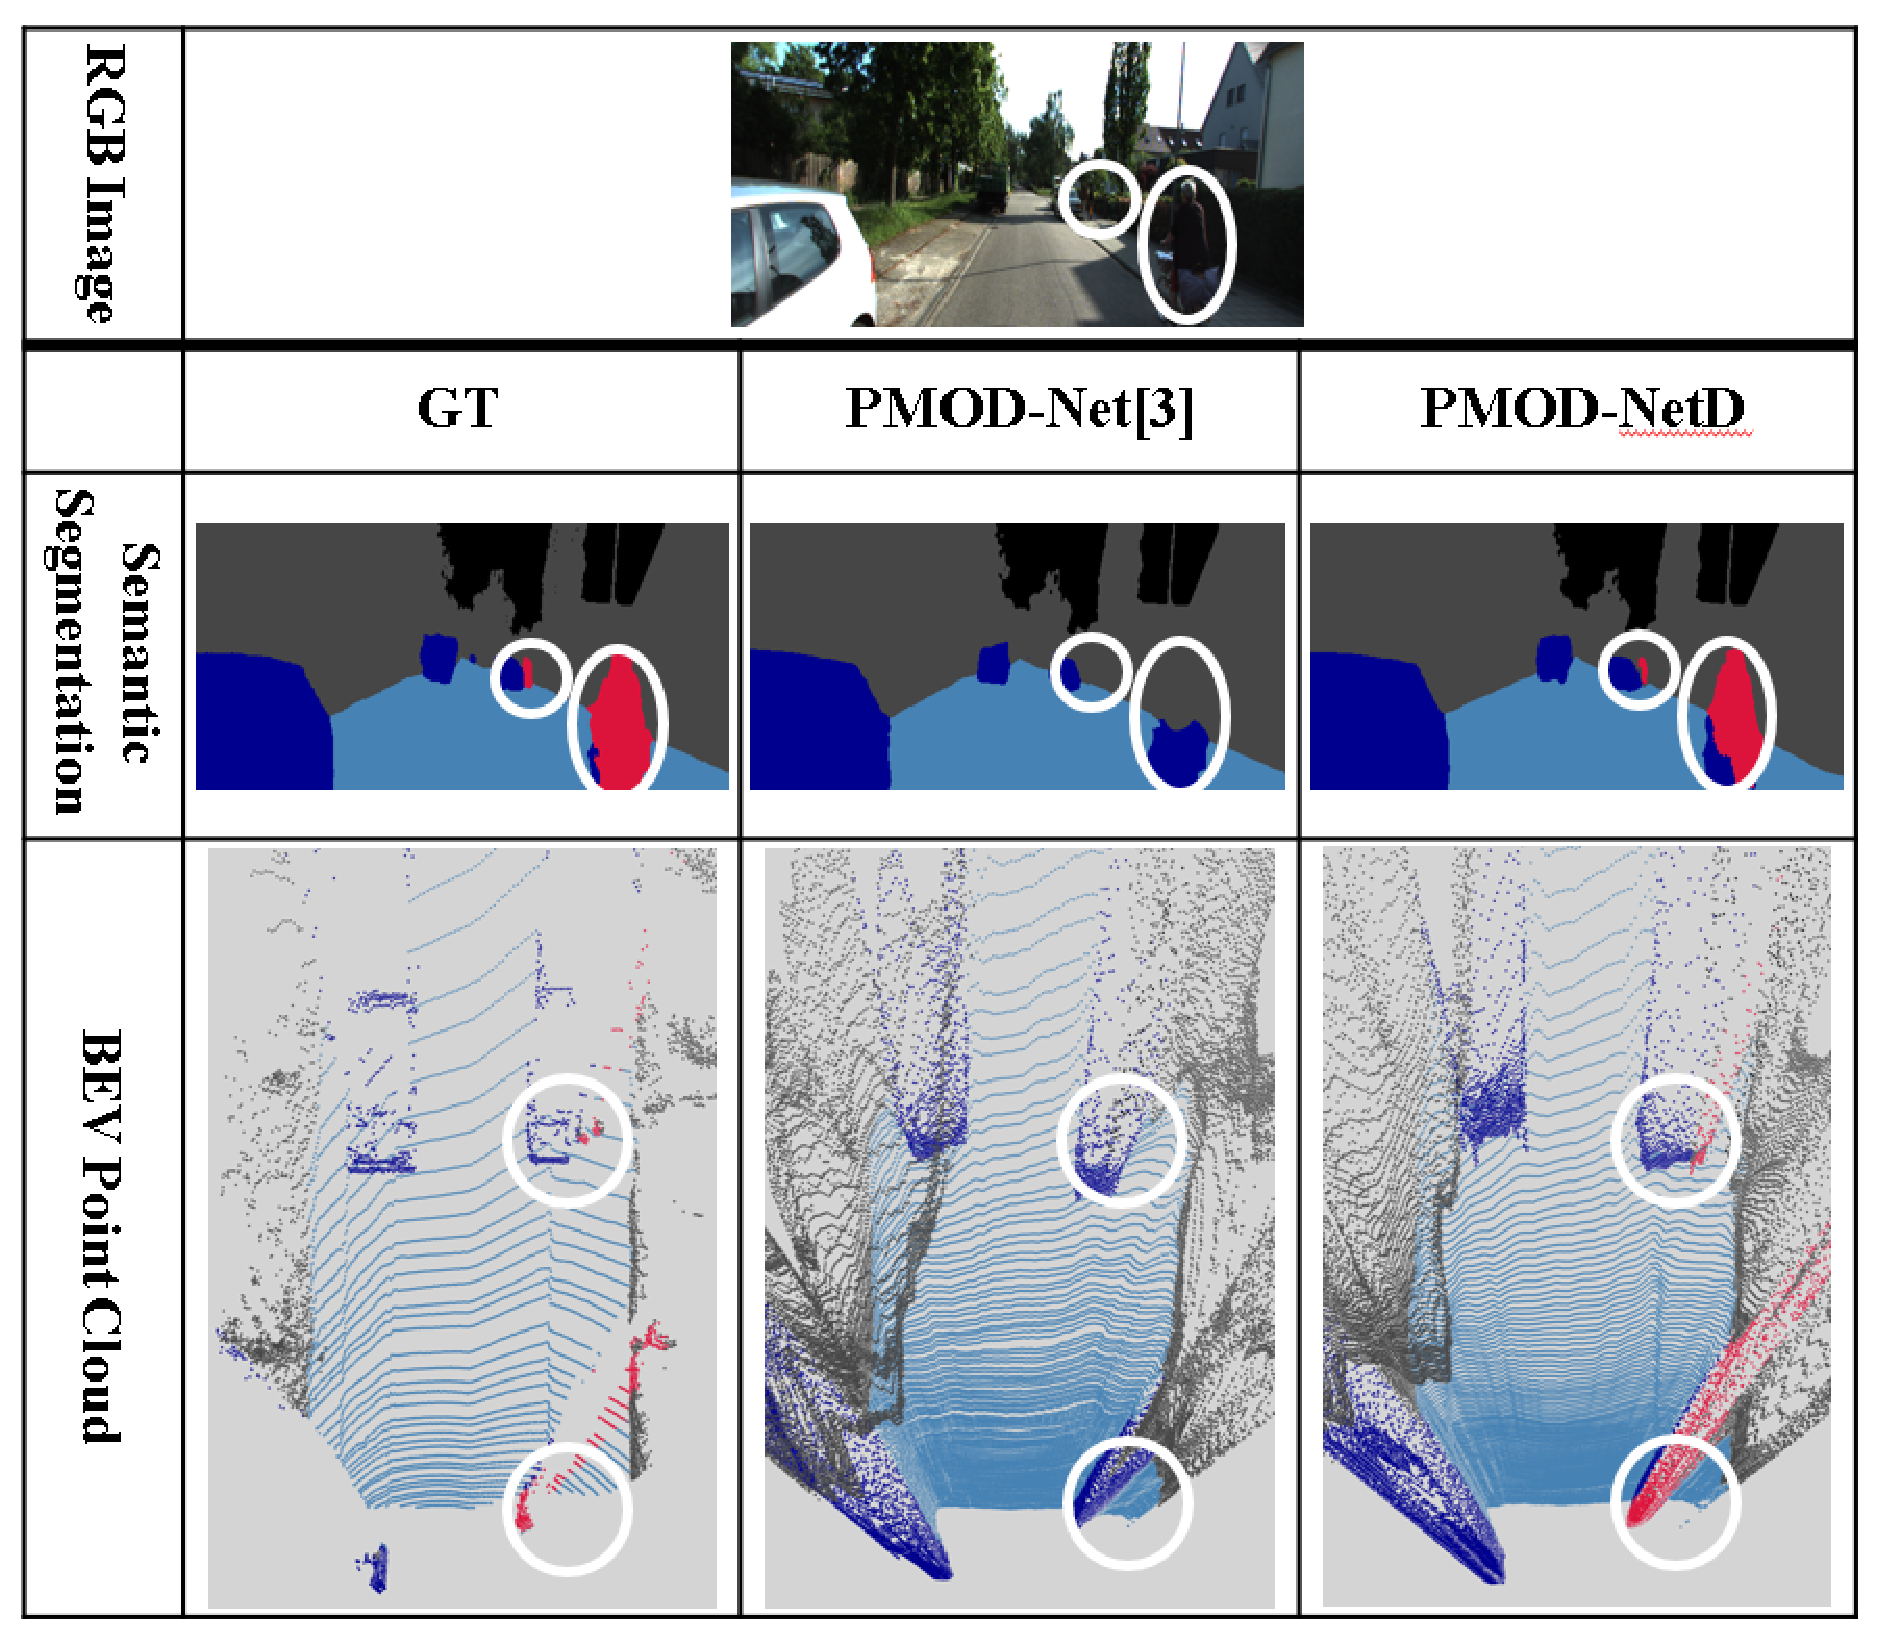
\includegraphics[width=0.935\linewidth]{img/evaluation/result_KITTI-360.eps}
  \caption{Experimental results in KITTI-360}
  \label{result_KITTI-360} 
\end{figure}

\reftable{result_MAE_CARLA}，\reftable{result_MAE_KITTI-360}の実験結果からPMOD-NetDはPMOD-Netよりも精度が向上していることが
わかった．新たに単眼深度画像を導入したことで，動的障害物の
距離推定精度向上に影響を与えたと考える．従来の PMOD-Net
では移動ロボットを利用した低速自動運転において，約2.8m
の間隔で配置された障害物の回避を実現している\cite{3}．本手法はPMOD-Netより精度向上
したため，さらに狭い間隔で障害物が配置された複雑な環境での自動運転に貢献できると
考えられる．

さらに\reffig{result_KITTI-360}のSegmentation結果
を見るとPMOD-Netでは検出できていない人が検出できていることもわかる．
単眼深度推定で障害物の境界を明確にすることは，セグメンテーション結果
にも有用であることが考察された．またNDDepthを用いた場合もMIMDepthを
用いた場合も，元の単眼深度推定結果よりもPMOD-NetDの方が高精度となった．
精度が良いMIMDepthを基にしたPMOD-NetDの方が，より精度が高い．したがって
今後高精度な単眼深度推定が開発された際に，PMOD-NetDに応用することで，
さらなる高精度化が期待できる．

しかし鳥瞰図を見ると，障害物の後方への距離推定誤差がまだ大きいことがわかる．
距離的に遠方にある背景の影響が強いため，障害物の境界を
強調して学習する損失などの導入が必要である．

\reftable{result_ME_CARLA}，\reftable{result_ME_KITTI-360}の実験結果から，本提案手法では，推定位置が正解より手前か奥かといっ
た傾向がデータセットごとに異なることがわかる．データセット内に含まれる物体の距離
の分布によって傾向が異なると考えられるため，手前に推定させたい場合は，データセット
に含まれる物体までの距離を全体的に短くするなど，学習させる距離の分布を調整するこ
とは重要である．

